
\breaksection{Scenario I: Business-as-usual}\label{sec:bau}

\iconBAUbig

\subsection{Context}

\boxquote{green}{\textbf{Can the Supply of Natural Resources Really Be Infinite? Yes!} \newline
Hold your hat --- our supplies of natural resources are not finite in any economic sense. Nor does past experience give reason to expect natural resources to become more scarce. Rather, if history is any guide, \textbf{natural resources will progressively become less costly, hence less scarce}, and will constitute a smaller proportion of our expenses in future years. Population growth is likely to have a long-run beneficial impact on the natural-resource situation.}{Julian Lincoln Simon in \textit{The Ultimate Resource}~\cite{simon1998ultimateresource2,simon1983ultimateresource}}

\boxquote{red}{Population growth, along with over-consumption per capita, is driving civilisation over the edge: billions of people are now hungry or micronutrient malnourished, and climate disruption is killing people. [Societal collapse] is a near certainty in the next few decades, and the risk is increasing continually as long as perpetual growth of the human enterprise remains the goal of economic and political systems. As I've said many times, \textbf{`perpetual growth is the creed of the cancer cell'}}{Paul Ehrlich~\cite{guardian2018ehrlich}, see also~\cite{ehrlich1978ecoscience,ehrlich1986popbomb, ehrlich2009popbombrevisited}}

\subsection{Storyline narrative}
This scenario envisions the future based on the current situation, extending to 2050 with very little deviation from present consumption patterns and the secondary raw material (SRM) system~\cite{iea2022worldenergyoutlook}. While there may be advances in some areas such as resource efficiency, recovery technology, and the energy transition, substantial modifications remain hindered by economic, social, and political constraints. The primary extraction of raw materials continues to be the primary source to meet the EU's demand.

In the Business As Usual (BAU) scenario, we are projecting the trajectory of the present into the future, extending up to the mid-century mark, 2050, with minimal disruption to existing consumption habits and the secondary raw material (SRM) system. This scenario unfolds on the assumption that the current pace and direction of technological, economic, and social development continue unhindered, and is characterised by a strong persistence of today's patterns.

In this scenario, we see moderate improvements in resource efficiency, advancements in recovery technology, and a slow transition towards greener energy sources. However, these developments are only minor tweaks to the existing system, failing to disrupt or fundamentally alter the established structure. The potential for transformational change remains largely untapped due to various hurdles. Economic constraints, social resistance to change, political inertia, and entrenched interests act as barriers to change, stifling efforts toward a more sustainable SRM system.

Primary extraction of raw materials remains the dominant source for raw materials consumed in the EU, continuing the linear `take-make-dispose' model of resource consumption (see \autoref{fig:linearmodel}). Base metals are well recycled, given their developed markets and economies of scale but rare/special metals are wasted because recycling technologies and economics do not allow for their recovery. Recycling and recovery rates remain stubbornly low, resulting in significant CRM waste. Meanwhile, material demand continues to rise in tandem with GDP growth, further exacerbating the resource pressure.


\begin{figure}[h!]
  \centering
  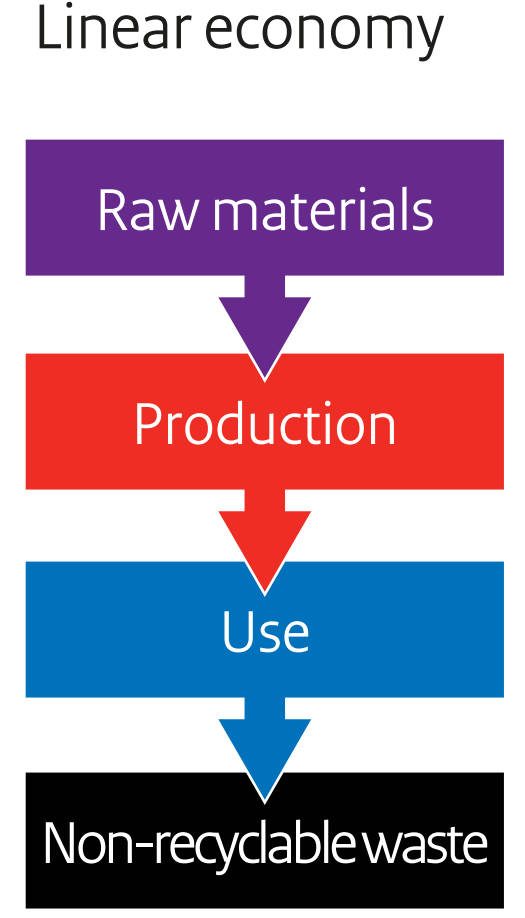
\includegraphics[height=7cm]{120storylines/nl2016ce-linear.png}
  \caption[The linear economy model in the business-as-usual scenario]{The linear economy model in the business-as-usual scenario~\cite{nl2016ceplan}}
  \label{fig:linearmodel}
\end{figure}


Moreover, the environmental impacts of mining and extraction persist as a significant concern. These operations continue to degrade ecosystems, leading to loss of biodiversity and contributing to climate change~\cite{ipcc2024climate}. Simultaneously, the EU becomes increasingly dependent on imports of SRMs, raising concerns about supply chain security and geopolitical risks~\cite{ipcc2024climate}.

Innovation in SRM recovery technologies is hampered by a lack of investment and regulatory support. The focus remains predominantly on cost-effective material production and use, with little regard for environmental implications or long-term sustainability. Material scarcity and price fluctuations, therefore, may become a considerable risk to the EU industry, limiting stable penetration of new recovery technology and threatening economic stability.

Moreover, the tightening of environmental regulations is restricted, inadequately addressing emerging challenges or incentivising sustainable practices. The lack of regulatory progress may further exacerbate environmental damage and biodiversity loss.

In essence, the BAU scenario is characterised by a continuation of current trends and practices, a future where the potential for a sustainable SRM system is unrealised due to the stranglehold of prevailing economic, social, and political constraints.

In the Business-as-usual (linear economy) scenario, the following are key characteristics:

\begin{itemize}
  \item A forecasting model is used to predict the future based on the current situation and the development of existing trends.
  \item Many EU targets for recycling and recovery are not met, and the current linear model largely persists.
  \item Material demand keeps pace with GDP growth, perpetuating a trend of increasing consumption. Primary mining and extraction persist as the leading sources of raw materials, underlining the dependency on traditional extraction methods.
  \item Recycling and recovery rates continue to lag, leading to an accumulation of SRM waste that signals missed opportunities for resource reuse.
  \item The environmental repercussions of mining and extraction, such as land degradation and water pollution, continue to be a pressing concern, reflecting the ecological toll of this linear model.
  \item The EU's dependency on imports of SRMs escalates, heightening the risk of supply disruptions. While supply disruption can serve to stimulate investment in new SRM recovery, volatility stifles innovation and advancements in this field.
  \item The industrial focus remains on cost-effective material production and use, disregarding the long-term sustainability aspect.
\end{itemize}

\subsectionEndline
\clearpage

\subsection{Waste stream specific scenario impacts}

\wasteSubsubsecBATT 
\textbf{Sources:}~\cite{helander2023battelv, eu2020batt, halleux2021batt, eu2023batt}

In the business-as-usual (BAU) scenario, the management of end-of-life batteries remains largely unchanged. The lack of technological innovation and regulatory incentives leads to a continued low recovery rate of valuable materials from battery waste.

\begin{itemize}
  \item A growing volume of battery waste due to the increased use of electronic transport and renewable energy storage systems.
  \item Lack of technological innovation and regulatory incentives lead to low recovery rates for certain battery types and certain elements.
  \item Collection systems for battery waste remain sporadic and unstandardised.
  \item Primary extraction remains the dominant source of battery materials.
  \item Share of LIB will increase (EV, LMT, Industrial LIB uptake)
  \item LIB Battery Chemistries will change and new LIB technologies will enter the market. Though, not with a focus on recycling and recovery.
  \item Larger portable batteries: shift towards Li-ion batteries
  \item Small format batteries in EEE: no significant change in battery chemistry.
  \item Use of critical resources continues but is already decreasing (BATT chemistry already changing towards less CRM content)
  \item Large-scale reuse of batteries is minimal
  \item Collection rates do not fulfil the EU targets
  \item Recycling efficiencies do not fulfil the EU targets
  \item Recovery rates do not fulfil the EU targets
\end{itemize}



\wasteSubsubsecELV
\textbf{Sources:}~\cite{eu2023elv,lovik2021elv, tazi2023elv,helander2023battelv,ljunggren2022elv,iea2023evoutlook}

The BAU scenario maintains the current approach to end-of-life vehicles, with minimal improvements in the recovery and recycling process. The absence of effective technologies and regulatory incentives results in low recovery rates of valuable materials from ELVs.

\begin{itemize}
  \item Legislation banning new ICEVs from 2035
  \item Current recovery technologies are unable to significantly improve the extraction of valuable materials from ELVs.
  \item Consumer demand continues to drive high production of new vehicles.
  \item ELV collection systems remain at their current efficiency.
  \item A significant proportion of vehicle components continue to end up as waste.
  \item Gradual and slow improvement of recycling chain technology efficiency
  \item No new legislation to improve recovery and support circular strategies in comparison to 2023
\end{itemize}



\wasteSubsubsecWEEE
\textbf{Sources:}~\cite{parajuly2019weee,un2023weee,forti2020weee,eu2012weee,eu2012weeerecast, narbonperpina2020weee}

In the BAU scenario, the treatment of WEEE does not significantly change. The lack of technological progress and effective regulation results in low recovery rates of valuable materials from WEEE.

\begin{itemize}
  \item Limited improvements in the recovery of valuable materials from WEEE.
  \item High consumer demand for new electronics continues to drive high WEEE generation.
  \item Ineffective collection systems and lack of public interest result in significant amounts of WEEE ending up in landfills.
  \item No significant growth in collaboration between government and industry for WEEE recovery.
  \item The majority of WEEE continues to be treated with common domestic waste, with low recycling rates.
  \item No groundbreaking technologies and practices to improve recovery and circularity.
  \item Reuse of products and components is not widely utilised
  \item Changes in legislation (e.g., circular economy and product design targets, targets for collection and recycling) are not strictly implemented.
  \item The BAU and the REC scenarios are similar from the put-on-market perspective (e.g., production and consumption remain the same), but it`s the recovery stage that makes the difference.
\end{itemize}



\wasteSubsubsecMIN
\textbf{Sources:}

The BAU scenario sees the continuation of current practices in mining waste management. The absence of advanced recovery technologies and regulatory incentives leads to low recovery rates of valuable materials from mining waste.

\begin{itemize}
  \item Limited technological advancements lead to static recovery rates of valuable materials from mining waste.
  \item Continued reliance on primary extraction as the dominant source of raw materials.
  \item Minimal advances in collaboration between government and industry for mining waste recovery.
  \item Low levels of traceability and management of mining waste.
  \item Mining waste remains a significant environmental challenge.
  \item Mining waste recovery projects remain too expensive.
  \item Little incentive for the private sector and public sector, except for monitoring environmental risks of existing deposits.
\end{itemize}



\wasteSubsubsecCDW
\textbf{Sources:}~\cite{eu2008wastedirective}

In the BAU scenario, the management of Construction and Demolition Waste (CDW) remains largely unchanged.

\begin{itemize}
  \item Focus on new construction to meet demand, no changes in CDW generation rate.
  \item No increase or refurbishment or renovation activities relative to new construction rates.
  \item Continue meeting the 2020 EU target from the Waste Directive~\cite{eu2008wastedirective} of 70\% CDW recovery (including preparation for re-use, recycling, and other material recovery, including backfilling)
  \item Recovery of metals remains on already high levels (\>90\%)~\cite{moschen2023cdw}.
  \item Recovery of minerals remains on already high levels (\>70\%) by using them as aggregates in road construction and backfilling~\cite{moschen2023cdw}.
  \item Recycling of wind turbines stays around 85\% (mainly metals), permanent magnets continue to be recycled as part of the metal fractions.[CITATION]
  \item Base metals are recovered as they have been, though there are limited improvements in recovery technologies and regulatory incentives.
  \item Repowering trends for wind turbines persist.
  \item Excluding wind turbines, there is no particular focus on the recovery of CRMs from CDW, where they constitute only a small fraction of the total mass (e.g., embedded in scrap steel).
        % \item Renovation as an alternative to new construction is not widely adopted.
\end{itemize}



\wasteSubsubsecSLASH 
\textbf{Sources:}~\cite{eurofer2023steel,euroal2023aluminium,vogl2020steelgreen,visualcapitalist2023steel,asquer2019ash}

In the BAU scenario, SLASH continues to be treated generally as low or negative-value waste. The absence of economically profitable recovery technologies or regulatory mandates leads to low improvements in the recovery rates of CRMs from SLASH.

\subsubsubsection{Slags}

Slags are waste products from the metallurgical industry and contain mainly minerals with some metals that could not be recovered during the metallurgical process. The reasons the metals are not recovered are:

\begin{enumerate}
  \item Current technology does not allow further recovery
  \item The metals are not of economic interest.
\end{enumerate}

More than 90\% of the slags are minerals, therefore the slags that are in line with the environmental criteria (end of waste criteria) are valorised as aggregates for the construction industry or as SCM (cement replacement materials). 

Slags containing high concentrations of heavy metals are landfilled. 

\begin{itemize}
  \item The volume of slags will stay stable. From 2013-2023, there was a stable production of metals, which results in a stable production of slags.  
  \item Due to the energy transition, it is expected the volume of slags from "classic" furnaces (eg BOF) will reduce and the number of slags from electric arc furnace will go up.
  \item  There are limited facilities to recover CRMs/SRMs, but the metallurgical companies do their best to recover as much of the metals as per their economic interests.
\end{itemize}

\subsubsubsection{Ashes}

Ashes are the waste products from the incineration of fossil fuels, biomass, or waste. We distinguish two main types: fly ashes and bottom ashes. Coal fly ashes are used as SCM to replace cement up to 30\%. Biomass (bottom and fly) ashes are used (based on the composition) as fertilizer or landfilled. Fly ashes from waste incineration are landfilled, while the bottom ashes are --- depending on the location in the EU --- further treated. 

The fractions that are rich in ferrous metals, aluminium, copper, and zinc are separated and used as input materials for the Fe, Cu, Zn, Al industries. By processing the Cu-rich fractions, PGMs, Ag, and Au are also recovered. The main part of the bottom ashes consists of mineral aggregates, which are used in the construction industry (when they are in line with the environmental criteria). In case the ashes are not treated (or only partly treated), they will be landfilled. 


\begin{itemize}
  \item In the last 10--20 years in some EU countries, we have seen a shift from landfilling towards incineration. This will lead to an increase in the volume of ashes from waste incineration.
  \item There was a drop in the use of coal as a fuel source, so the volume of coal ashes dropped over the last 10 years and is expected to drop further. 
  \item At the same time the volume of biomass incineration went up. It is uncertain if this volume will increase in the future further (due to the high pressure on land that is needed to produce this biomass).
  \item Almost all coal fly ashes are used as SCM (high-value stream up to 80 EUR/ton). 
  For Biomass fly ashes there are no sorting facilities, while for waste inceration bottom ashes, there are sorting installations in place, but for the moment, they are not present in all EU  countries, and therefore, there is still room for improvement. 
  \item 
\end{itemize}


% \begin{itemize}
%   \item Increased generation of SLASH because SRMs are not recovered and end up in incineration and smelter residues.
%   \item Low quality of SLASH due to:
%         \begin{itemize}
%           \item poor sorting and separation of waste streams (e.g., consumer electronics and batteries, end up in general waste streams and are incinerated)
%           \item high `contamination' from the above-described failures of segregation.
%           \item large proportion coming from mixed waste incineration
%         \end{itemize}
%   \item Lack of technological advancements results in low recovery rates of valuable materials from SLASH.
%   \item Continued high generation of SLASH due to the reliance on traditional energy sources.
%   \item Minimal incentives for the recovery and reuse of materials from SLASH.
%   \item Low levels of traceability and management of SLASH.
%   \item SLASH continues to be a significant environmental challenge due to the high volume generated.
%   \item Some products from SLASH are recovered in low added value, for example, as aggregates for roads or additives in cement.
% \end{itemize}

\sectionEndlines

\breaksection{Scenario II: Recovery}\label{sec:rec}

\iconRECbig

\subsection{Context}

\boxquote{green}{
  We are in a period of economic transition. The `cowboy economy' of the past is
  obsolescent, if not obsolete. Environmental services are no longer free goods, and this fact is driving major changes. Recycling is the wave of the (immediate) future. \textbf{The potential savings in terms of energy and capital have long been obvious. The savings in terms of reduced environmental impact are less obvious but increasingly important.} The obstacle to greater use recycling has been the fact that economies of scale still favor large primary mining and smelting complexes over (necessarily) smaller and less centralized recyclers. But this advantage is declining over time as the inventory of potentially recyclable metals in industrialized society grows to the point that efficient collection and logistic systems, and efficient markets, justify significant investments in recycling. \textbf{Increasing energy and other resource costs, together with increasing costs of waste treatment and disposal, will favor this shift in any case.} But government policies, driven by unemployment and environmental concerns, taken together, may accelerate the shift by gradually reducing taxes on labor and increasing taxes
  on extractive resource use.
}{Robert U. Ayres~\cite{ayres1997recycling}}

\boxquote{red}{
  One does not require much of an imagination to picture how complex it is to physically and chemically separate these components again to ultimately retrieve the metals. \textbf{It's just about as difficult as recycling your morning cup of coffee into its ingredients\ldots} There are no simple answers here --- at some point, the amount of effort also outweighs the value of the metal content. This knowledge should prompt a consciousness shift in our utilization of our limited resources\ldots \newline
  \textbf{The inconvenient truth is that closing the loop is impossible!} Therefore, an honest discussion involves speaking transparently about losses in the process: in the form of energy, metals, and dust, for example. There are technological and economic limits to closing the loop.
}{Prof. Dr. Dr. h.c. mult. Markus Reuter \cite{reuter2019aurubis}}



\subsection{Storyline narrative}

In the recovery scenario, the central emphasis is on harnessing sophisticated technologies to salvage SRMs from waste streams at the end of their lifecycle. While there are noticeable strides towards the incorporation of `circular design' principles and re-X strategies, they are mostly seen at the end-of-life and material demand is akin to that observed in the BAU scenario. This is, however, mitigated by the implementation of a comprehensive material recovery system. \autoref{fig:reusemodel} presents a simplified visual depiction of the dominant material flow paths in the recovery scenario.


\begin{figure}[h!]
  \centering
  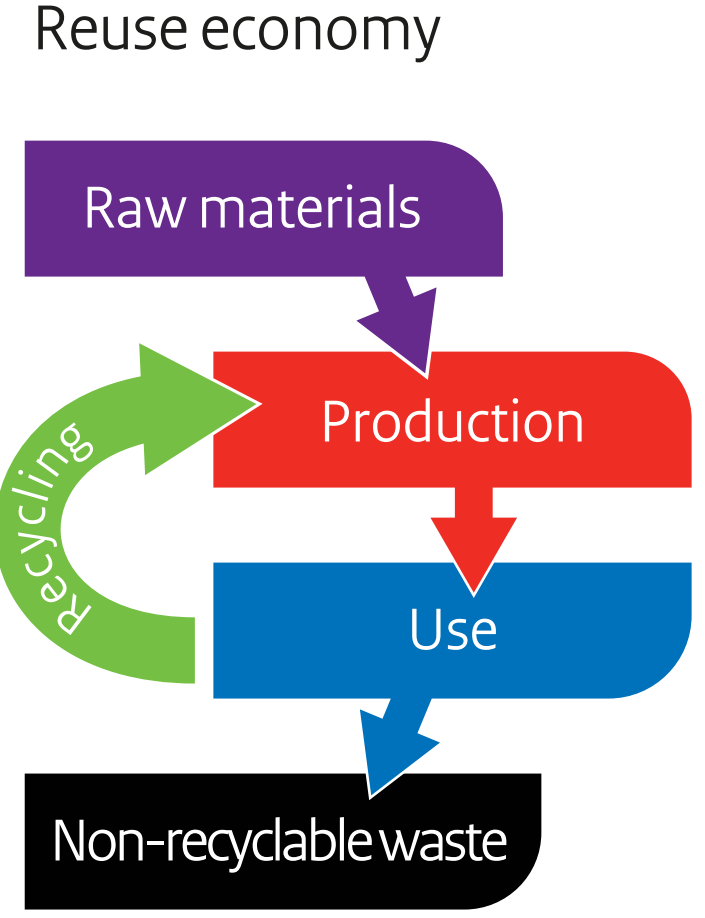
\includegraphics[height=7cm]{120storylines/nl2016ce-reuse.png}
  \caption[The reuse economy model in the recovery scenario]{The reuse economy model in the recovery scenario~\cite{nl2016ceplan}}
  \label{fig:reusemodel}
\end{figure}

In this scenario, the central actor is the waste treatment sector, with the spotlight falling on the enhancement of recovery technology. The implementation and optimisation of cutting-edge technologies, such as Artificial Intelligence (AI), automation, and advanced robotics, play a significant role in revolutionising waste treatment processes. These technologies streamline waste sorting, improve the quality of recovered materials, and increase the overall efficiency of the recovery process.

This scenario calls for an emphasis on policy development and standardisation to foster EU-wide development, integration, and compliance. Here, the role of governments and policy-makers becomes crucial in setting more ambitious recovery targets, developing conducive regulatory frameworks, and enforcing compliance. This multi-pronged approach also involves strengthening cross-border cooperation, harmonising waste management standards, and promoting knowledge and technology transfer among EU member states.

To realise more ambitious environmental impact reduction targets, significant progress needs to be made in both technological and policy aspects. Enhancing technological capabilities will improve recovery rates, while robust policy measures will ensure these advancements are integrated into the wider economy in a regulated manner. The future of this scenario depends on the successful fusion of advanced technology, regulatory harmonisation, and a commitment to continuous improvement in waste management and SRM recovery.

Key characteristics of this technology-promoted recovery scenario include:

\begin{itemize}
  \item This scenario uses a combination of forecasting and backcasting methods to envision the future.
  \item The backcasting method is used for scenario factors that are covered by governmental targets, starting with the desired outcome and working backwards to the present.
  \item The forecasting method is used for scenario factors that are not covered by governmental targets, starting with the current situation and extending to the future.
  \item EU targets for recycling and recovery are met, due to the EU's waste management system becoming more expansive, efficient and effective.
  \item Technological innovation drives increased recovery rates of SRMs, enabling the more efficient use of waste.
  \item Digitalisation and automation are more extensively used in recycling processes, leading to enhanced productivity and accuracy.
  \item There is greater exploration and exploitation of alternative sources such as urban mining, waste streams, and tailings, presenting novel opportunities for resource acquisition.
  \item New waste regulations and guidelines for SRM recovery are implemented, enforcing better management and extraction of SRMs.
  \item Investment in research and development for SRM recovery technologies experiences an upswing, promoting continuous innovation in this field.
  \item Closer collaboration and information sharing between industry and government institutions streamline processes and expedite decision-making.
  \item New jobs are created in the recycling and recovery sector, offering economic benefits and improving overall employment rates.
  \item SRM production and use become more efficient and cost-effective, fostering economic sustainability.
  \item Environmental impact from mining and extraction is reduced, signalling a more sustainable approach to resource acquisition.
  \item The EU's dependence on primary extraction is reduced, with SRM recovery becoming a more significant source of raw materials.
\end{itemize}

\subsectionEndline
\clearpage

\subsection{Waste stream specific scenario impacts}



\wasteSubsubsecBATT
\textbf{Sources:}~\cite{helander2023battelv, eu2020batt, halleux2021batt, eu2023batt}

Under the recovery scenario, end-of-life batteries become a crucial source of secondary raw materials, primarily due to the increased adoption of electric vehicles and renewable energy storage systems. Technological innovation drives the recovery and recycling process, ensuring valuable materials are extracted from waste batteries for reuse.

\begin{itemize}
  \item Increase in end-of-life batteries due to the growth of electric vehicles and renewable energy storage.
  \item Advanced recovery technologies facilitate the efficient extraction of valuable materials from battery waste.
  \item Standardised collection systems enhance the quantity and quality of battery waste available for recovery.
  \item Industry and government collaboration lead to investments in research and development of battery recovery technologies.
  \item Battery passports have a strong impact on collection, material recovery rates and recycling rates.
  \item Collection
        \begin{itemize}
          \item Portable battery collection increases according to the trend seen in the WEEE waste stream.
          \item Improved collection of light means of transport (LMT) batteries.
          \item Improved regulation and collection of Industrial batteries.
        \end{itemize}
  \item Material recovery
        \begin{itemize}
          \item Improved recycling technologies
          \item Battery Pass will improve material recovery
          \item Higher recovery rate for lithium
          \item Increase in recycling by average weight
          \item Recycling of plastics
        \end{itemize}
  \item Ambitious goals of recycling/recovery rates compete with reuse, so reuse remains low.
  \item Improved public awareness means that fewer batteries end up in the municipal waste stream and there is less hoarding.
  \item Against this: there is competition for the batteries from the reuse vs. recycling market.
  \item Design for recycling (DFR):
        \begin{itemize}
          \item Material and composition selection for recycling~\cite{helander2023battelv}.
          \item Higher requirements on disassemblability.
          \item Information available to promote efficient recovery.
        \end{itemize}
\end{itemize}



\wasteSubsubsecELV 
\textbf{Sources:}~\cite{eu2023elv,lovik2021elv, tazi2023elv,helander2023battelv,ljunggren2022elv, iea2023evoutlook}

The recovery scenario envisions a more effective and technology-driven end-of-life vehicle treatment process. Advancements in recovery technologies allow for improved extraction of valuable materials from vehicles at their end of life, although consumerism still drives high demand for new vehicles.

\begin{itemize}
  \item Innovations in recovery technologies allow for a higher recovery rate of CRM-containing materials from ELVs.
  \item The total number of vehicles produced remains high due to consumer demand.
  \item Improved systems for ELV collection are established, ensuring efficient management of ELV waste.
  \item Increased collaboration between the government and industry leads to investments in ELV recovery technologies.
  \item Focus on managing end-of-life of vehicles
  \item EU recovery targets are reached (currently implemented/proposed targets, but also increased and new targets)
  \item Common/bulk materials (Fe, Non-Fe, plastics etc.,) and precious metals (Au, Ag, Pd, Pt) reach high mass recycling rates and high element recycling rates. Other CRMs currently not recovered reach a moderate level of recovery.
  \item For instance,
        \begin{itemize}
          \item More advanced dismantling and processing steps (e.g., components and materials)
          \item More specialised recovery of certain components and materials (e.g., electric motors including permanent magnets and embedded REE) as suggested in the proposal for a revised ELV directive.
          \item More public and private interest in developing recycling chains
          \item Increase in collection rate due to increase in participation from the public and businesses, i.e., target-based incentives with strong regulations and monitoring
        \end{itemize}
  \item Design for recycling (DFR):
        \begin{itemize}
          \item Higher requirements on `disassemblability'.
          \item Information available to enable recovery.
        \end{itemize}
\end{itemize}



\wasteSubsubsecWEEE 
\textbf{Sources:}~\cite{parajuly2019weee,un2023weee,forti2020weee,eu2012weee, eu2012weeerecast, narbonperpina2020weee}

Under the recovery scenario, WEEE becomes a significant resource for secondary raw materials. Technological advancements in the sector improve the efficiency of WEEE treatment, although the consumerism-driven demand for new electronics remains high.

\begin{itemize}
  \item Advanced technologies enable higher recovery rates of valuable materials from WEEE
  \item Despite advancements in design for recyclability, WEEE generation remains high due to the consumer demand for new electronics
  \item Standardised and segregated collection systems for WEEE are implemented, improving the supply of materials for recovery
  \item Increased industry-government collaboration leads to further development in WEEE recovery technologies
  \item Consumer behaviour remains a significant hurdle for more efficient WEEE management
  \item Higher recycling rate --- make full use of the disposed parts. For instance:
        \begin{itemize}
          \item more automation of the dismantling and processing steps (e.g., AI)
          \item recycling technologies improvements (e.g., small components recovery is also happening)
          \item more effective collection infrastructure
          \item financial support provided to recyclers/operators
          \item bans on WEEE exports push for increased domestic recycling~\cite{huisman2015weee}
        \end{itemize}
  \item `Design for recovery' principle --- Ecodesign mandates changes in weight and composition of EEE so complexity and the type of materials used
  \item Higher public awareness and participation on WEEE issue and management
  \item Higher compliance from the public, the producers and the businesses
  \item Strong regulations and monitoring are in place with higher collection and recycling targets which are set and implemented and fines are set for those who fail to achieve the targets
  \item Focus is given more to the EoL management of WEEE
\end{itemize}



\wasteSubsubsecMIN 
\textbf{Sources:} 

Under the recovery scenario, technological advancements enable the extraction of residual valuable materials from mining waste, transforming it into a more valuable resource.

\begin{itemize}
  \item Technological advancements facilitate the extraction of valuable materials from mining waste.
  \item Despite progress in recovery technologies, primary extraction remains the dominant source of raw materials due to high consumer demand.
  \item Government and industry collaboration support the development of technologies for the recovery of materials from mining waste.
  \item Increased traceability and management of mining waste through digitalisation.
  \item Mining waste remains a significant environmental challenge.
\end{itemize}

\wasteSubsubsecCDW 
\textbf{Sources:}~\cite{eu2008wastedirective}

Under the recovery scenario, Construction and Demolition Waste (CDW) becomes an important resource for secondary raw materials, though mostly base metals and aggregates. Despite some progress in eco-design and material efficiency, the construction industry continues to generate significant amounts of waste or `downcycled' materials. Some progress in eco-design and material efficiency, but the construction industry continues to generate significant amounts of waste or ‘downcycled’ materials.

\begin{itemize}
  \item Focus on new construction to meet demand, no changes in CDW generation rate.
  \item No increase or refurbishment or renovation activities.
        % \item Advanced recovery technologies allow for higher recovery rates of valuable materials from CDW.
        % \item Eliminating the disposal of any avoidable CDW, through the implementation and expansion of incentives and regulatory measures.
        % \item The focus of this scenario is to reduce the amount of CDW that ends up in treatment plants without any useful applications, e.g., landfilling, incineration, and land spreading.
  \item Enhancement of the quality of recycling to recover materials at higher value.
  \item Increased investment and enhanced regulatory system in waste management, contributing to increased recovery.
  \item Creation of new waste recovery infrastructure that improves recovery.
  \item Widespread application of selective demolition and strict on-site waste sorting leasing to an increase in recovery of waste.
        % \item This scenario is characterized by a high recovery rate, achieved via:
        % \begin{itemize}
        %   \item increased investment and enhanced regulatory system in waste management,
        %   \item leading to more waste recovery infrastructure,
        %   \item widespread application of selective demolition and on-site waste sorting.
        % \end{itemize}.
  \item Recovery of minerals is intensified with a stronger focus on closed-loop recycling (e.g., cement and aggregate are separated, aggregate is used, but cement is not treated).
  \item Recovery of other materials like glass, plastics, and wood is also intensified.
  \item Better separation of waste at source leads to a higher quality of secondary raw materials.
  \item Repowering trends for wind turbines stay the same.
  \item Improved recycling of wind turbine blades is notable, especially regarding plastics; permanent magnets are recycled at a functional level.
\end{itemize}



\wasteSubsubsecSLASH 
\textbf{Sources:}~\cite{eurofer2023steel,euroal2023aluminium,vogl2020steelgreen,visualcapitalist2023steel,asquer2019ash}

In the recovery scenario, SLASH are recognized as a potential resource for secondary raw materials. Advances in recovery technologies enable the extraction of valuable metals from SLASH, however, the total volume of CRMs recovered from this material remains low, except in cases of supply constraint.

\begin{itemize}
   \item Digital solutions enhance the traceability and management of SLASH.
   \item More functional collection infrastructure.
   \item Financial support provided to recyclers/operators.
   \item Introduction of SRM/CRM recovery targets. For example, recovery of P from biomass ash for fertilizer.
   \item Higher awareness and participation of relevant sectors on SLASH issues and management.
   \item Strong regulations and monitoring are in place with higher collection and recycling targets.
 \end{itemize}

\subsubsubsection{Slags}


\begin{itemize}
\item Advanced recovery technologies allow for the extraction of valuable metals and minerals from slags.
\item New recovery technologies are installed in the metallurgical industry. 
\item All metals are recovered from the slags, and the slag itself only contains minerals or metals as trace elements.
\item Due to the low metal content, the slags are ideal resources for the construction industry.
\end{itemize}

\subsubsubsection{Ashes}
\begin{itemize}
\item New recovery technologies are installed in the incineration industry.
\item We expect a shift in the volume and quality of the ashes.
\item Coal fly ashes are the same as in BAU reducing over time to almost zero.
\item Biomass ashes have the same volume and quality.
\item Waste incineration ashes: due to the recovery scenario there will be a shift from landfill and incineration towards recycling,  reuse, and repair. In countries with a high landfill rate, this will lead to higher volumes of ashes. In countries with a low landfill rate, and a high volume of incineration: this will lead to lower volumes of ashes, and a shift in the composition (with less CRM content in the ashes, due to better pre-sorting)
\end{itemize}


\sectionEndlines

\breaksection{Scenario III: Circularity}\label{sec:cir}

\iconCIRbig

\subsection{Context}


\boxquote{green}{
  A circular economy is one that is regenerative by design and aims to keep products, components, and materials at their highest utility and value at all times, distinguishing between technical and biological cycles. This new economic model seeks to ultimately decouple global economic development from finite resource consumption.}{Ellen MacArthur Foundation~\cite{ellenmacarthur2015ce}}


\boxquote{green}{
  \textbf{A Circular Economy in the Netherlands by 2050!} \newline
  Imagine we are in the year 2050. In the Netherlands we are living within the planetary boundaries of the Earth rather than permanently crossing them. This is because our relationship with nature, which used to be highly disturbed and led to climate change, has changed for the better \ldots \newline \ldots~The Netherlands now has a circular economy. \newline\ldots~The Dutch Government intends to achieve a fully circular economy by 2050 and to halve the use of primary abiotic raw materials by 2030.}
{National Circular Economy Programme, Government of the Netherlands~\cite{nl2023ceplan}}


\boxquote{red}{
\textbf{Circularity of the Dutch economy has barely increased} \newline
Of all natural resources that were deployed in the Dutch economy in 2020, 13 percent consisted of recycled materials. This percentage is virtually the same as in 2014. In terms of recycling, the circularity of the Dutch economy has barely increased.}{CBS (Statistics Netherlands)~\cite{cbs2023circularity}}

\boxquote{red}{
  The circular economy promises radical technological transformations in a couple of decades, ``nothing less than to open up new and immense horizons for industry'', ``provide multiple value creation mechanisms'', produce ``better welfare, GDP, and employment outcomes''~\cite{ellenmacarthur2015ce}. Looking at these claims, one wonders whether policymakers really believe that in 30 years EU citizens will live in an inclusive economy with zero waste, zero emissions, with a perpetual economic growth, continuously absorbing massive flows of immigrants while protecting and enhancing the ecological processes and environmental biodiversity. \newline

  \ldots for a young scientist it is not advisable and even shocking to say in policy circles that:
  \begin{enumerate}[label=(\roman*)]
    \item Reaching zero emissions for metabolic systems is impossible (open/living systems must breathe),
    \item The economic process is entropic and therefore a circular economy enabling perpetual economic growth is impossible (it is the biosphere and not the technosphere that recycles matter, while energy cannot be recycled), and
    \item The existing technosphere has been built on and relied on fossil fuels for over 200 years, and it cannot be completely replaced in 30 years reaching zero emissions while fulfilling all the sustainable development goals (including rapid economic growth in the developing world).
  \end{enumerate}
}{M. Giampietro and S.O. Funtowicz~\cite{giampietro2020cecritique}}


\subsection{Storyline narrative}

A circular economy focuses on significantly enhancing resource efficiency. This can be achieved through four primary strategies:
\begin{enumerate}
    \item Minimizing resource use (narrowing the loop) through shared utilization or opting out of certain product use, along with improved manufacturing efficiencies;
    \item Prolonging the life and utility of products and their components (slowing the loop) via reuse and repair, thereby reducing the need for new raw materials;
    \item Recycling materials (closing the loop) to diminish the quantity of material incinerated or sent to landfills, consequently cutting down the demand for new raw materials;
    \item Replacing finite resources with renewable ones (like bioresources) or alternative primary resources that have a lower environmental impact.
\end{enumerate}

In this scenario, we move in the direction of the maximum achievable state of material efficiency as government policy, private innovation and social changes are rapidly driving the transition toward a circular economy. The emphasis here rests heavily on re-X strategies that are implemented in the design phase of products (e.g., repairability and re-manufacturability) and that are actualised by changes in consumer behaviour (e.g reduction, refusal, engagement in the `sharing economy' and curtailment of the `throw-away' mindset).

\autoref{fig:circmodel} presents a simplified visual depiction of the dominant material flow paths in the recovery scenario.


\begin{figure}[h!]
  \centering
  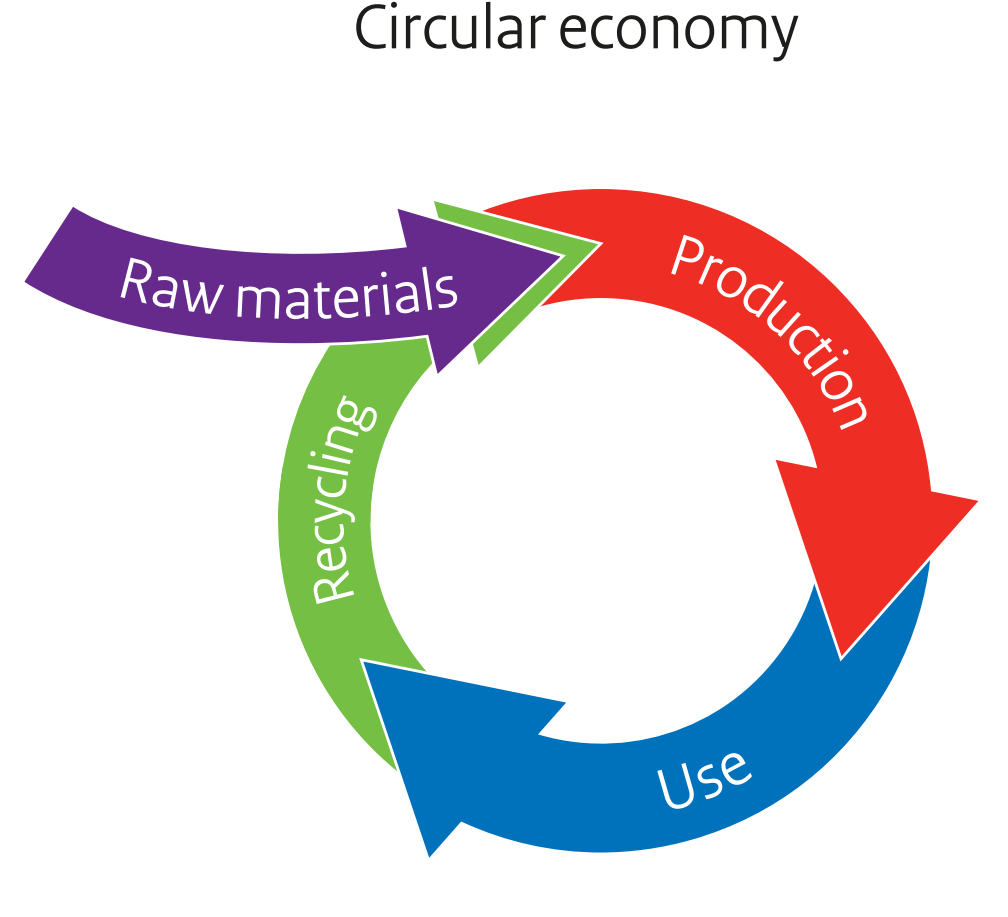
\includegraphics[height=7cm]{120storylines/nl2016ce-circ.png}
  \caption[The simplified circular economy model in the circularity scenario]{The simplified circular economy model in the circularity scenario~\cite{nl2016ceplan}}
  \label{fig:circmodel}
\end{figure}


Further, being enabled by the widespread adoption of `circular design' principles and improvements in information transparency (e.g., waste tracking and digital product passports) the system for the treatment of post-consumer waste can divert a significant amount of their inflows (to, for example, re-use and re-manufacture) with the residual fraction being readily segregated into purer, more efficiently recoverable, material streams.

This scenario envisions a future where government policies are in synergy with private sector innovation and societal changes, driving a wholesale transition towards a circular economy. Unlike the recovery scenario, where the focus is on the end-of-life recovery of materials, this scenario emphasises minimising waste at all stages, starting from the design phase itself, where both policymakers and designers are moving away from short-lived products towards products designed for longevity.


The emphasis is on re-X strategies that are integrated throughout the entirety of a product's lifecycle. This includes repairability, where products are designed to be easily fixed rather than replaced; and re-manufacturability, where products or their components are designed to be restored to their original state, extending their lifespan and reducing the need for new resources. This scenario calls for a drastic change in consumer behaviour, where reduction in consumption and waste, refusal of non-sustainable options, and active participation in the `sharing economy' become the norm rather than the exception.

In the circularity scenario, the widespread adoption of `circular design' principles becomes a cornerstone of production. In a circular design approach, products are designed and produced in a way that considers their entire lifecycle, including eventual disassembly and reuse. New economic models make it costly for producers to generate short-lived products and material waste. Companies are now giving priority to the design of products that are easily repairable, can be disassembled, and reused. The rise of technology has paved the way for predictive maintenance tools. These allow businesses to keep a tab on material conditions through sensors and carry out repairs before a malfunction occurs, a method gaining traction in transport and manufacturing.

Additionally, this scenario envisions an improvement in transparency, with measures such as waste tracking and digital product passports becoming standard. Waste tracking allows for efficient management of waste flows, aiding in effective resource planning, while digital product passports provide information about a product`s composition and how it can be properly disassembled, reused, or recycled. Material composition, including raw materials, is transparent to all involved in the value chain, promoting closer collaboration. Producers see the advantage of being open about their product details to aid in repair, repurposing, and recycling activities. This transparency about product components, durability, and reparability increases consumer demand for products that are designed to last and can be reused or recycled.


\subsectionEndline

\subsection{Scenario needs and impacts}

In the proposed scenario, the European Union (EU) embarks on a pivotal transition towards a circular economy. This framework emphasises the retention of product, material, and resource value within the economic matrix for extended durations, simultaneously minimising waste generation. This transition is integral to the EU's strategic goal of cultivating a sustainable, low-carbon, resource-efficient, and globally competitive economy.

The implications of this shift are multifaceted. It presents an avenue for the EU to rejuvenate its economic architecture while providing businesses with a protective shield against challenges such as resource scarcity and price volatility. This revised economic model fosters the emergence of efficient, innovative production and consumption methods, thus offering novel business opportunities. Moreover, the circular economy approach has palpable socio-economic benefits, including diverse job creation and enhanced social integration.

From an environmental perspective, the transition aids in the reduction of the cumulative energy footprint and helps mitigate irreversible ecological damages. This encompasses challenges related to climate shifts, biodiversity conservation, and comprehensive pollution control. Several studies accentuate the overarching benefits of this economic approach, highlighting potential reductions in prevalent carbon dioxide emissions.

The successful implementation of this vision necessitates a collaborative approach involving various stakeholders, encompassing businesses, consumers, and regulatory entities. A robust regulatory framework is indispensable, designed to promote optimal practices and delineate clear progression benchmarks. This comprehensive framework encompasses the entirety of the circular economy's value chain, from production to consumption, extending into realms of repair, remanufacturing, and waste management, culminating in the reintroduction of secondary raw materials into the economic cycle.

Environmental fiscal reforms are crucial for a circular economy transition. Taxes should pivot from labour to resource depletion, promoting a double dividend. The EU can leverage the VAT directive and the European semester process to endorse flexible rates on circular services like repair. It's imperative to abolish harmful subsidies, notably on fossil fuels, which are inherently linear and which Member States have pledged to eliminate. The tax framework should incentivise pioneers challenging the established linear economy. Analysing tax shifts at the national level can determine tax effectiveness and pinpoint instruments that best bolster circularity.

The contribution of member states is paramount. They play a dual role, both in the actualisation of EU directives and in the integration of complementary regional initiatives. The principles of a circular economy possess global applicability, necessitating harmonised strategies within the EU and with external international partners. Such synergised efforts are crucial for the fulfilment of broader international commitments, notably the U.N. 2030 Agenda for Sustainable Development~\cite{un2015sdg}. The ultimate objective remains the establishment of a sustainable future characterised by judicious consumption and production protocols.

\subsectionEndline
\clearpage

\subsection{Waste stream specific scenario impacts}


\wasteSubsubsecBATT 
\textbf{Sources:}~\cite{helander2023battelv, eu2020batt, halleux2021batt, eu2023batt}


In the circularity scenario, battery waste treatment undergoes a massive transformation. The shift towards electric vehicles and renewable energy storage significantly increases the quantity of end-of-life batteries. However, thanks to new regulations, technological advancements, and business models, the majority of battery components are recycled or reused.

\begin{itemize}
  \item Massive increase in end-of-life batteries due to the shift to electric vehicles and renewable energy storage.
  \item New regulations incentivise battery manufacturers to design for recycling.
  \item Battery recycling technologies improve, enabling higher recovery rates of valuable metals.
  \item Standardised collection systems for battery waste are established, improving the efficiency of the recycling process.
  \item Service-based business models like leasing ensure manufacturers retain ownership of the batteries, promoting circularity.
  \item Greater transparency through digital product passports aids in effective battery waste management.
  \item Battery passport and publicly accessible Information from the new Battery Regulation (SoH, SoC, Predicted lifetime/warranty, etc.) given by the economic operator that places the battery on the market enables high re-use rates.
  \item Increased repairability/modularity.
  \item Reduced demand from `sharing economy’ and more `sustainable’ transport choices.
  \item New emerging technologies more suited for reuse/repair.
  \item Ambitious targets set by business and public policy.
\end{itemize}



\wasteSubsubsecELV 
\textbf{Sources:}~\cite{eu2023elv,lovik2021elv, tazi2023elv, helander2023battelv, ljunggren2022elv,iea2023evoutlook}


For End-of-Life Vehicles (ELVs), the circular economy model affects the way vehicles are designed, used, and discarded. Emphasising extended vehicle life through repair and remanufacturing, this scenario also focuses on the recovery of materials from vehicles at the end of their life.

\begin{itemize}
  \item Vehicle design shifts towards repairability, upgradability, and recyclability, increasing the lifespan of vehicles.
  \item Standardised systems for ELV collection are established, ensuring efficient waste management.
  \item Innovative technologies enable higher recovery rates of metals and other valuable materials from ELVs.
  \item Service-based models like vehicle leasing and sharing could reduce the total number of vehicles produced.
  \item Digital product passports provide information about vehicle components, aiding in effective recycling or reuse.
  \item Focus on managing the use-phase of vehicles.
  \item Circular strategies take place before material recovery so that material recovery is “delayed”.
  \item Information available to enable these strategies.
  \item EU vehicles policy has implications for materials in vehicles, such as `lightweighting' and downsizing
        \begin{itemize}
          \item Increase in average occupancy and average vehicle-kilometres per trip.
          \item Decrease in average lifetime (in terms of years): As the utilisation factor increases.
        \end{itemize}
  \item Increase in circular strategies due to an increase in participation from the public and businesses, i.e., target-based incentives with strong regulations and monitoring.
\end{itemize}



\wasteSubsubsecWEEE 
\textbf{Sources:}~\cite{parajuly2019weee,un2023weee,forti2020weee,eu2012weee, eu2012weeerecast, narbonperpina2020weee}


In the circularity scenario, WEEE becomes a valuable resource instead of a disposal challenge. Thanks to product design changes and the application of advanced recovery technologies, a significant percentage of the materials in WEEE is reclaimed and fed back into the production cycle.

\begin{itemize}
  \item Electronic products are designed for longevity, repairability, upgradability, and recyclability.
  \item Advanced technologies enable higher recovery rates of precious metals from WEEE.
  \item Collection systems for WEEE are improved, ensuring a steady supply of materials to feed the recovery system.
  \item Digitalisation and data use enhance traceability and efficiency in WEEE management.
  \item Service-based models for electronics promote the use of products as a service rather than ownership, reducing WEEE generation~\cite{geissdorfer2020circbusinessmodels}.
  \item Increased durability and lifespans.
  \item Increased repairability.
  \item More sharing and product-service systems, correspond to a reduction in the lifetime (for some equipment).
  \item More reuse practices (expanded second-hand market).
  \item Less hoarding.
  \item Higher formal collection and recycling rate.
  \item Focus is given more to the production and use phase rather than the EoL (End-of-Life).
  \item `Design for circularity' principle: Ecodesign mandates repairability, durability, no obsolescence, modularity, and that continual software upgrades are possible~\cite{eu2023chargers, eu2023chargerspress}.
  \item Electronically compatible chargers and battery packs can be used by different products.
  \item The above also means that chargers and batteries are not integrated into the product and that the product is designed to be easily disassembled.
  \item Strong regulations and monitoring are in place with higher reuse and circular targets, which are set and implemented, and fines are imposed on the member states that fail to achieve the targets.
  \item Support and development of circular strategies infrastructure (e.g., easy information access for repairability, repair shops, accessibility to spare components on the market, etc.).
  \item Greater use of connected products, smart technologies, and the IoT. Used to monitor and diagnose product performance in situ which, can extend product and component life.
\end{itemize}



\wasteSubsubsecMIN 
\textbf{Sources:}


In this scenario, the impact on mining waste is two-fold. Firstly, the need for primary mining is reduced due to lower demand, efficient resource use and high recovery rates of materials. Secondly, mining waste itself is treated as a valuable resource, with advanced technologies being used to extract residual valuable materials.

\begin{itemize}
  \item A Decrease in primary mining reduces the generation of mining waste.
  \item Advanced technologies are employed to extract valuable materials from mining waste.
  \item Policies and regulations incentivise the reuse of mining waste in various applications.
  \item Digital solutions improve tracking and management of mining waste.
  \item Collaboration between stakeholders promotes circular practices in the mining industry.
\end{itemize}


\wasteSubsubsecCDW 
\textbf{Sources:}~\cite{eu2008wastedirective}

Construction and Demolition Waste (CDW) is another sector that sees significant improvement in the circularity scenario. This scenario reduces the generation of CDW and promotes the recovery of valuable materials from the waste stream.


\begin{itemize}
  \item Less demolition and new construction results in a reduction of CDW.
  \item Buildings are designed for disassembly and reuse, increasing the lifespan of materials and reducing CDW.
  \item Longer lifetimes for buildings (more renovation and refurbishment) and wind turbines (less repowering, i.e. changing of wind turbines before the end of theoretical lifespan).
  \item Wind turbine blades are  refurbished or repaired and then reused.
  \item Recycling technologies for CDW improve, allowing higher recovery rates of materials and less `downcycling'.
  \item Policies and regulations incentivise the use of recycled materials in construction.
  \item Standardised systems for CDW collection and separation are improved.
  \item Digital tools like building information modelling (BIM) improve resource management in construction and renovation.
  \item Focus on dismantling and selective deconstruction: constructions are taken apart in a way that individual parts can be reused.
        % \item This scenario envisions an almost closed-loop system where CDW is considered a resource, with an emphasis on minimising waste generation and maximising resource efficiency in recovery.
        % \item Waste reduction is prioritized through the implementation of eco-designs, including designing out waste (DOW), lightweight design (LWD), and design for dismantling (DFD).
        % \item Reuse and repair standards and networks are established to boost the reuse of end-of-life building components and equipment.
        % \item If reuse is no longer possible, waste is recycled through high-efficiency recycling facilities rather than down-cycled or used for energy recovery.
        % \item Plausible target: Achieving a 100\% recovery rate of avoidable CDW by 2050, with a recycling rate accounting for 30\% and component reuse accounting for 20\%. Raw material consumption should be reduced by 50\% compared to the 2020 level.
        % \item Example of treatment technological development: Waste concrete is primarily recycled through an innovative mobile dry process. Biodiesel-based thermal treatment is applied to further pyrolyze the fine aggregate to recover cement. Lightweight design is implemented to reduce concrete use.
\end{itemize}


\wasteSubsubsecSLASH 
\textbf{Sources:}~\cite{eurofer2023steel,euroal2023aluminium,vogl2020steelgreen,visualcapitalist2023steel,asquer2019ash}


% In the circularity scenario, the approach to SLASH dramatically changes. Instead of being treated as waste, SLASH is seen as a valuable secondary raw material. Advances in technology allow for the extraction of valuable metals and minerals from SLASH, that then re-enter the material cycle.

% \begin{itemize}
%   \item A shift in perception treats SLASH as a valuable resource instead of waste.
%   \item Advanced technologies enable the extraction of valuable metals and minerals from SLASH.
%   \item New regulations incentivise the use of SLASH in various applications, such as in the construction industry.
%   \item Digital solutions enhance the tracking and management of SLASH.
%   \item Collaboration between industries utilises SLASH in new and innovative ways.
%   \item Reduce the generation of SLASH by increasing the efficiency of the manufacturing side. For example, developing higher efficient production of metals and reducing by-products such as smelter slag.
%   \item For ash from the incineration of solid biomass, maximizing the use of biomass by setting proper temperature, time, and furnace conditions to reduce ash contents and improve the efficiency of power and heat generation.
%   \item For ash, developing other renewable technologies from bioenergy to reduce the incineration of solid biomass, e.g., biogas.
%   \item Reduce the generation of SLASH by increasing the proportion of higher calorific waste and decreasing lower calorific waste, e.g., MSW (Municipal Solid Waste).
%   \item Developing domestic feedstock supply for bioenergy or metal production to reduce the cost of transportation and others.
%   \item Higher formal collection and recycling rate compared to BAU, but lower compared to the Recovery scenario.
% \end{itemize}


In the circularity scenario, SLASH are recognised as a potential resource for secondary raw materials. Advances in recovery technologies enable the extraction of valuable metals from SLASH, however, the total volume of CRMs recovered from this material remains low, except in cases of supply constraint. In the circularity scenario, the conditions are very similar to that of the recovery scenario, except that volumes will decrease, due to a general decrease in waste generation.

\begin{itemize}
   \item Digital solutions enhance the traceability and management of SLASH.
   \item More functional collection infrastructure.
   \item Financial support provided to recyclers/operators.
   \item Introduction of SRM/CRM recovery targets. For example, recovery of P from biomass ash for fertiliser.
   \item Higher awareness and participation of relevant sectors on SLASH issues and management.
   \item Strong regulations and monitoring are in place with higher collection and recycling targets.
 \end{itemize}

\subsubsubsection{Slags}
\begin{itemize}
\item Advanced recovery technologies allow for the extraction of valuable metals and minerals from slags.
\item New recovery technologies are installed in the metallurgical industry. 
\item All metals are recovered from the slags, and the slag itself only contains minerals or metals as trace elements.
\item Due to the low metal content, the slags are ideal resources for the construction industry.
\end{itemize}

\subsubsubsection{Ashes}
\begin{itemize}
\item New recovery technologies are installed in the incineration industry.
\item We expect a shift in the volume and quality of the ashes.
\item Coal fly ashes are the same as in BAU reducing over time to almost zero.
\item Biomass ashes have the same volume and quality.
\item Waste incineration ashes: due to the recovery scenario there will be a shift from landfill and incineration towards recycling,  reuse, and repair. In countries with a high landfill rate, this will lead to higher volumes of ashes. In countries with a low landfill rate, and a high volume of incineration: this will lead to lower volumes of ashes, and a shift in the composition (with less CRMs in the ashes, due to better pre-sorting)
\end{itemize}
